% Options for packages loaded elsewhere
\PassOptionsToPackage{unicode}{hyperref}
\PassOptionsToPackage{hyphens}{url}
\PassOptionsToPackage{dvipsnames,svgnames,x11names}{xcolor}
%
\documentclass[
  letterpaper,
  DIV=11,
  numbers=noendperiod]{scrartcl}

\usepackage{amsmath,amssymb}
\usepackage{iftex}
\ifPDFTeX
  \usepackage[T1]{fontenc}
  \usepackage[utf8]{inputenc}
  \usepackage{textcomp} % provide euro and other symbols
\else % if luatex or xetex
  \usepackage{unicode-math}
  \defaultfontfeatures{Scale=MatchLowercase}
  \defaultfontfeatures[\rmfamily]{Ligatures=TeX,Scale=1}
\fi
\usepackage{lmodern}
\ifPDFTeX\else  
    % xetex/luatex font selection
\fi
% Use upquote if available, for straight quotes in verbatim environments
\IfFileExists{upquote.sty}{\usepackage{upquote}}{}
\IfFileExists{microtype.sty}{% use microtype if available
  \usepackage[]{microtype}
  \UseMicrotypeSet[protrusion]{basicmath} % disable protrusion for tt fonts
}{}
\makeatletter
\@ifundefined{KOMAClassName}{% if non-KOMA class
  \IfFileExists{parskip.sty}{%
    \usepackage{parskip}
  }{% else
    \setlength{\parindent}{0pt}
    \setlength{\parskip}{6pt plus 2pt minus 1pt}}
}{% if KOMA class
  \KOMAoptions{parskip=half}}
\makeatother
\usepackage{xcolor}
\setlength{\emergencystretch}{3em} % prevent overfull lines
\setcounter{secnumdepth}{-\maxdimen} % remove section numbering
% Make \paragraph and \subparagraph free-standing
\makeatletter
\ifx\paragraph\undefined\else
  \let\oldparagraph\paragraph
  \renewcommand{\paragraph}{
    \@ifstar
      \xxxParagraphStar
      \xxxParagraphNoStar
  }
  \newcommand{\xxxParagraphStar}[1]{\oldparagraph*{#1}\mbox{}}
  \newcommand{\xxxParagraphNoStar}[1]{\oldparagraph{#1}\mbox{}}
\fi
\ifx\subparagraph\undefined\else
  \let\oldsubparagraph\subparagraph
  \renewcommand{\subparagraph}{
    \@ifstar
      \xxxSubParagraphStar
      \xxxSubParagraphNoStar
  }
  \newcommand{\xxxSubParagraphStar}[1]{\oldsubparagraph*{#1}\mbox{}}
  \newcommand{\xxxSubParagraphNoStar}[1]{\oldsubparagraph{#1}\mbox{}}
\fi
\makeatother

\usepackage{color}
\usepackage{fancyvrb}
\newcommand{\VerbBar}{|}
\newcommand{\VERB}{\Verb[commandchars=\\\{\}]}
\DefineVerbatimEnvironment{Highlighting}{Verbatim}{commandchars=\\\{\}}
% Add ',fontsize=\small' for more characters per line
\usepackage{framed}
\definecolor{shadecolor}{RGB}{241,243,245}
\newenvironment{Shaded}{\begin{snugshade}}{\end{snugshade}}
\newcommand{\AlertTok}[1]{\textcolor[rgb]{0.68,0.00,0.00}{#1}}
\newcommand{\AnnotationTok}[1]{\textcolor[rgb]{0.37,0.37,0.37}{#1}}
\newcommand{\AttributeTok}[1]{\textcolor[rgb]{0.40,0.45,0.13}{#1}}
\newcommand{\BaseNTok}[1]{\textcolor[rgb]{0.68,0.00,0.00}{#1}}
\newcommand{\BuiltInTok}[1]{\textcolor[rgb]{0.00,0.23,0.31}{#1}}
\newcommand{\CharTok}[1]{\textcolor[rgb]{0.13,0.47,0.30}{#1}}
\newcommand{\CommentTok}[1]{\textcolor[rgb]{0.37,0.37,0.37}{#1}}
\newcommand{\CommentVarTok}[1]{\textcolor[rgb]{0.37,0.37,0.37}{\textit{#1}}}
\newcommand{\ConstantTok}[1]{\textcolor[rgb]{0.56,0.35,0.01}{#1}}
\newcommand{\ControlFlowTok}[1]{\textcolor[rgb]{0.00,0.23,0.31}{\textbf{#1}}}
\newcommand{\DataTypeTok}[1]{\textcolor[rgb]{0.68,0.00,0.00}{#1}}
\newcommand{\DecValTok}[1]{\textcolor[rgb]{0.68,0.00,0.00}{#1}}
\newcommand{\DocumentationTok}[1]{\textcolor[rgb]{0.37,0.37,0.37}{\textit{#1}}}
\newcommand{\ErrorTok}[1]{\textcolor[rgb]{0.68,0.00,0.00}{#1}}
\newcommand{\ExtensionTok}[1]{\textcolor[rgb]{0.00,0.23,0.31}{#1}}
\newcommand{\FloatTok}[1]{\textcolor[rgb]{0.68,0.00,0.00}{#1}}
\newcommand{\FunctionTok}[1]{\textcolor[rgb]{0.28,0.35,0.67}{#1}}
\newcommand{\ImportTok}[1]{\textcolor[rgb]{0.00,0.46,0.62}{#1}}
\newcommand{\InformationTok}[1]{\textcolor[rgb]{0.37,0.37,0.37}{#1}}
\newcommand{\KeywordTok}[1]{\textcolor[rgb]{0.00,0.23,0.31}{\textbf{#1}}}
\newcommand{\NormalTok}[1]{\textcolor[rgb]{0.00,0.23,0.31}{#1}}
\newcommand{\OperatorTok}[1]{\textcolor[rgb]{0.37,0.37,0.37}{#1}}
\newcommand{\OtherTok}[1]{\textcolor[rgb]{0.00,0.23,0.31}{#1}}
\newcommand{\PreprocessorTok}[1]{\textcolor[rgb]{0.68,0.00,0.00}{#1}}
\newcommand{\RegionMarkerTok}[1]{\textcolor[rgb]{0.00,0.23,0.31}{#1}}
\newcommand{\SpecialCharTok}[1]{\textcolor[rgb]{0.37,0.37,0.37}{#1}}
\newcommand{\SpecialStringTok}[1]{\textcolor[rgb]{0.13,0.47,0.30}{#1}}
\newcommand{\StringTok}[1]{\textcolor[rgb]{0.13,0.47,0.30}{#1}}
\newcommand{\VariableTok}[1]{\textcolor[rgb]{0.07,0.07,0.07}{#1}}
\newcommand{\VerbatimStringTok}[1]{\textcolor[rgb]{0.13,0.47,0.30}{#1}}
\newcommand{\WarningTok}[1]{\textcolor[rgb]{0.37,0.37,0.37}{\textit{#1}}}

\providecommand{\tightlist}{%
  \setlength{\itemsep}{0pt}\setlength{\parskip}{0pt}}\usepackage{longtable,booktabs,array}
\usepackage{calc} % for calculating minipage widths
% Correct order of tables after \paragraph or \subparagraph
\usepackage{etoolbox}
\makeatletter
\patchcmd\longtable{\par}{\if@noskipsec\mbox{}\fi\par}{}{}
\makeatother
% Allow footnotes in longtable head/foot
\IfFileExists{footnotehyper.sty}{\usepackage{footnotehyper}}{\usepackage{footnote}}
\makesavenoteenv{longtable}
\usepackage{graphicx}
\makeatletter
\def\maxwidth{\ifdim\Gin@nat@width>\linewidth\linewidth\else\Gin@nat@width\fi}
\def\maxheight{\ifdim\Gin@nat@height>\textheight\textheight\else\Gin@nat@height\fi}
\makeatother
% Scale images if necessary, so that they will not overflow the page
% margins by default, and it is still possible to overwrite the defaults
% using explicit options in \includegraphics[width, height, ...]{}
\setkeys{Gin}{width=\maxwidth,height=\maxheight,keepaspectratio}
% Set default figure placement to htbp
\makeatletter
\def\fps@figure{htbp}
\makeatother

\KOMAoption{captions}{tableheading}
\makeatletter
\@ifpackageloaded{caption}{}{\usepackage{caption}}
\AtBeginDocument{%
\ifdefined\contentsname
  \renewcommand*\contentsname{Table of contents}
\else
  \newcommand\contentsname{Table of contents}
\fi
\ifdefined\listfigurename
  \renewcommand*\listfigurename{List of Figures}
\else
  \newcommand\listfigurename{List of Figures}
\fi
\ifdefined\listtablename
  \renewcommand*\listtablename{List of Tables}
\else
  \newcommand\listtablename{List of Tables}
\fi
\ifdefined\figurename
  \renewcommand*\figurename{Figure}
\else
  \newcommand\figurename{Figure}
\fi
\ifdefined\tablename
  \renewcommand*\tablename{Table}
\else
  \newcommand\tablename{Table}
\fi
}
\@ifpackageloaded{float}{}{\usepackage{float}}
\floatstyle{ruled}
\@ifundefined{c@chapter}{\newfloat{codelisting}{h}{lop}}{\newfloat{codelisting}{h}{lop}[chapter]}
\floatname{codelisting}{Listing}
\newcommand*\listoflistings{\listof{codelisting}{List of Listings}}
\makeatother
\makeatletter
\makeatother
\makeatletter
\@ifpackageloaded{caption}{}{\usepackage{caption}}
\@ifpackageloaded{subcaption}{}{\usepackage{subcaption}}
\makeatother

\ifLuaTeX
  \usepackage{selnolig}  % disable illegal ligatures
\fi
\usepackage{bookmark}

\IfFileExists{xurl.sty}{\usepackage{xurl}}{} % add URL line breaks if available
\urlstyle{same} % disable monospaced font for URLs
\hypersetup{
  pdftitle={Homework 4},
  pdfauthor={Marshall Nielsen},
  colorlinks=true,
  linkcolor={blue},
  filecolor={Maroon},
  citecolor={Blue},
  urlcolor={Blue},
  pdfcreator={LaTeX via pandoc}}


\title{Homework 4}
\usepackage{etoolbox}
\makeatletter
\providecommand{\subtitle}[1]{% add subtitle to \maketitle
  \apptocmd{\@title}{\par {\large #1 \par}}{}{}
}
\makeatother
\subtitle{Multiple Linear Regression}
\author{Marshall Nielsen}
\date{}

\begin{document}
\maketitle


\subsection{Data and Description}\label{data-and-description}

Measuring body fat is complex. One method involves submerging the body
in water and measuring displacement. A simpler, more accessible method
would be preferable. To develop such a method, researchers collected
data from 252 men, recording age (years), weight (pounds), height
(inches), and three body circumference measurements (neck, chest, and
abdomen, all in centimeters). Each participant's body fat percentage
(variable ``brozek'') was accurately estimated using underwater
weighing. The goal is to create a predictive model using these basic
variables, eliminating the need for water displacement measurements.

The dataset, \texttt{BodyFat.txt}, is available on Canvas. Download
\texttt{BodyFat.txt} and place it in the same folder as this
\texttt{.qmd} file.

\paragraph{\texorpdfstring{0. Replace the text ``\textless{} PUT YOUR
NAME HERE \textgreater{}'' (above next to ``author:'') with your full
name.}{0. Replace the text ``\textless{} PUT YOUR NAME HERE \textgreater'' (above next to ``author:'') with your full name.}}\label{replace-the-text-put-your-name-here-above-next-to-author-with-your-full-name.}

\paragraph{1. Read in the data set, and call the data frame ``bodyfat''.
Display a summary of the data. Remove the ``row'' column (which contains
row numbers) from the data
set.}\label{read-in-the-data-set-and-call-the-data-frame-bodyfat.-display-a-summary-of-the-data.-remove-the-row-column-which-contains-row-numbers-from-the-data-set.}

\begin{Shaded}
\begin{Highlighting}[]
\NormalTok{bodyfat }\OtherTok{\textless{}{-}} \FunctionTok{read.table}\NormalTok{(}\StringTok{"BodyFat.txt"}\NormalTok{, }\AttributeTok{header =} \ConstantTok{TRUE}\NormalTok{)}
\NormalTok{bodyfat }\OtherTok{\textless{}{-}}\NormalTok{ bodyfat }\SpecialCharTok{\%\textgreater{}\%} \FunctionTok{select}\NormalTok{(}\SpecialCharTok{{-}}\NormalTok{row)}
\FunctionTok{summary}\NormalTok{(bodyfat)}
\end{Highlighting}
\end{Shaded}

\begin{verbatim}
     brozek           age            weight          height     
 Min.   : 0.00   Min.   :22.00   Min.   :118.5   Min.   :64.00  
 1st Qu.:12.80   1st Qu.:35.50   1st Qu.:158.8   1st Qu.:68.38  
 Median :19.00   Median :43.00   Median :176.2   Median :70.00  
 Mean   :18.89   Mean   :44.86   Mean   :178.8   Mean   :70.32  
 3rd Qu.:24.55   3rd Qu.:54.00   3rd Qu.:196.9   3rd Qu.:72.25  
 Max.   :45.10   Max.   :81.00   Max.   :363.1   Max.   :77.75  
      neck           chest           abdom       
 Min.   :31.10   Min.   : 79.3   Min.   : 69.40  
 1st Qu.:36.40   1st Qu.: 94.3   1st Qu.: 84.55  
 Median :38.00   Median : 99.6   Median : 90.90  
 Mean   :37.98   Mean   :100.8   Mean   : 92.49  
 3rd Qu.:39.40   3rd Qu.:105.3   3rd Qu.: 99.20  
 Max.   :51.20   Max.   :136.2   Max.   :148.10  
\end{verbatim}

\paragraph{2. Display a scatterplot matrix of the
data.}\label{display-a-scatterplot-matrix-of-the-data.}

\begin{Shaded}
\begin{Highlighting}[]
\FunctionTok{plot}\NormalTok{(bodyfat)}
\end{Highlighting}
\end{Shaded}

\begin{center}

\includegraphics{HW_4_files/figure-pdf/unnamed-chunk-2-1.pdf}
\end{center}

\paragraph{\texorpdfstring{3. Based on the scatterplot matrix, briefly
explain which variables you think will be helpful for predicting brozek
and which variables you think will \emph{not} be helpful at predicting
brozek. Explain how the scatterplot helped determine your
answers.}{3. Based on the scatterplot matrix, briefly explain which variables you think will be helpful for predicting brozek and which variables you think will not be helpful at predicting brozek. Explain how the scatterplot helped determine your answers.}}\label{based-on-the-scatterplot-matrix-briefly-explain-which-variables-you-think-will-be-helpful-for-predicting-brozek-and-which-variables-you-think-will-not-be-helpful-at-predicting-brozek.-explain-how-the-scatterplot-helped-determine-your-answers.}

Looking at the scatterplots, I think that weight, neck, chest, and
abdomen are going to be the most helpful for predicting brozek, and that
age and height will be less helpful. I think so because those first four
show obvious positive trends when plotted against brozek, while the
others are more scattered or flat.

\paragraph{4. Create and print a correlation matrix (numeric or color-
and
shape-coded).}\label{create-and-print-a-correlation-matrix-numeric-or-color--and-shape-coded.}

\begin{Shaded}
\begin{Highlighting}[]
\FunctionTok{round}\NormalTok{(}\FunctionTok{cor}\NormalTok{(bodyfat), }\DecValTok{2}\NormalTok{)}
\end{Highlighting}
\end{Shaded}

\begin{verbatim}
       brozek   age weight height neck chest abdom
brozek   1.00  0.29   0.61  -0.02 0.49  0.70  0.81
age      0.29  1.00  -0.01  -0.24 0.11  0.17  0.23
weight   0.61 -0.01   1.00   0.49 0.83  0.89  0.89
height  -0.02 -0.24   0.49   1.00 0.33  0.24  0.20
neck     0.49  0.11   0.83   0.33 1.00  0.78  0.75
chest    0.70  0.17   0.89   0.24 0.78  1.00  0.92
abdom    0.81  0.23   0.89   0.20 0.75  0.92  1.00
\end{verbatim}

\begin{Shaded}
\begin{Highlighting}[]
\FunctionTok{corrplot}\NormalTok{(}\FunctionTok{cor}\NormalTok{(bodyfat), }\AttributeTok{type =} \StringTok{"upper"}\NormalTok{)}
\end{Highlighting}
\end{Shaded}

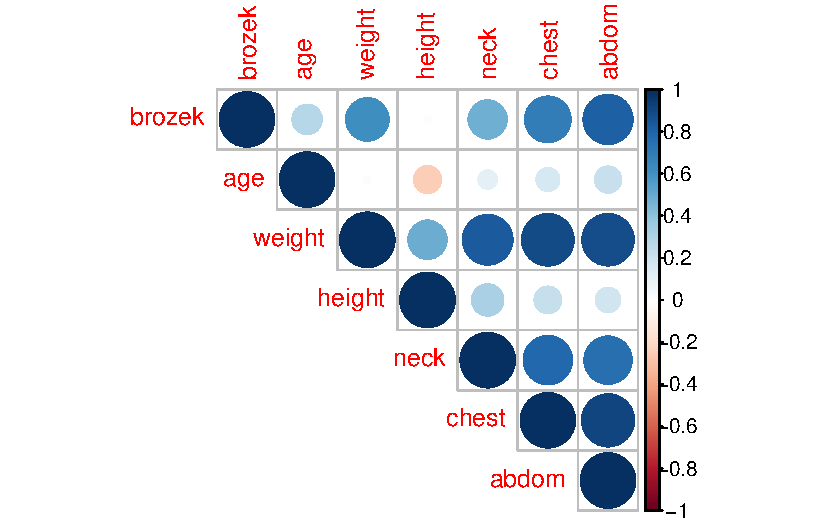
\includegraphics{HW_4_files/figure-pdf/unnamed-chunk-3-1.pdf}

\paragraph{5. Based on the scatterplot matrix and the correlation
matrix, are their any pairs of variables that you suspect will cause a
problem in terms of multicollinearity? If so, which
ones?}\label{based-on-the-scatterplot-matrix-and-the-correlation-matrix-are-their-any-pairs-of-variables-that-you-suspect-will-cause-a-problem-in-terms-of-multicollinearity-if-so-which-ones}

There are at least a few. The most worrisome would probably be weight
compared with neck, chest, or abdomen, neck with chest or abdomen and
chest with abdomen.

\paragraph{6. Fit a multiple linear regression model to the data (no
transformations). Display a summary of the
results.}\label{fit-a-multiple-linear-regression-model-to-the-data-no-transformations.-display-a-summary-of-the-results.}

\begin{Shaded}
\begin{Highlighting}[]
\NormalTok{linear\_model }\OtherTok{\textless{}{-}} \FunctionTok{lm}\NormalTok{(}\AttributeTok{data =}\NormalTok{ bodyfat, }\AttributeTok{formula =}\NormalTok{ brozek }\SpecialCharTok{\textasciitilde{}}\NormalTok{ .)}
\FunctionTok{summary}\NormalTok{(linear\_model)}
\end{Highlighting}
\end{Shaded}

\begin{verbatim}

Call:
lm(formula = brozek ~ ., data = bodyfat)

Residuals:
     Min       1Q   Median       3Q      Max 
-11.5811  -3.0358   0.0668   2.8879  10.2828 

Coefficients:
              Estimate Std. Error t value Pr(>|t|)    
(Intercept) -2.010e+01  1.413e+01  -1.423   0.1561    
age          5.010e-03  2.540e-02   0.197   0.8438    
weight      -8.733e-02  3.879e-02  -2.251   0.0253 *  
height      -1.400e-01  1.520e-01  -0.921   0.3579    
neck        -4.421e-01  2.019e-01  -2.189   0.0295 *  
chest        4.844e-04  9.107e-02   0.005   0.9958    
abdom        8.754e-01  7.924e-02  11.048   <2e-16 ***
---
Signif. codes:  0 '***' 0.001 '**' 0.01 '*' 0.05 '.' 0.1 ' ' 1

Residual standard error: 4.124 on 244 degrees of freedom
Multiple R-squared:  0.722, Adjusted R-squared:  0.7151 
F-statistic: 105.6 on 6 and 244 DF,  p-value: < 2.2e-16
\end{verbatim}

\paragraph{7. Briefly comment on the ``significance'' of the variables:
were you surprised by the results? Are there any variables that are
significant that you think shouldn't be? Are there any variables that
are not significant that you think should
be?}\label{briefly-comment-on-the-significance-of-the-variables-were-you-surprised-by-the-results-are-there-any-variables-that-are-significant-that-you-think-shouldnt-be-are-there-any-variables-that-are-not-significant-that-you-think-should-be}

It makes sense that weight and abdomen would be significant, but it
doesn't seem like neck should be over some of the other variables
measured. I also feel like chest should be significant as well.

\paragraph{8. Briefly comment on the sign (+/-) of the coefficients for
the variables. Are their any variables where the sign is the opposite of
what you
expected?}\label{briefly-comment-on-the-sign---of-the-coefficients-for-the-variables.-are-their-any-variables-where-the-sign-is-the-opposite-of-what-you-expected}

Definitely. Weight for one is currently displaying a negative
coefficient when it should probably be positive. Neck should also be
positive in general even if it isn't the strongest predictor in the set.

\paragraph{\texorpdfstring{9. Mathematically write out the \emph{fitted}
multiple linear regression model for this data set using the
coefficients you found above (do not use \(\beta\)s). Do not use ``X''
and ``Y'' in your model - use variable names that are
descriptive.}{9. Mathematically write out the fitted multiple linear regression model for this data set using the coefficients you found above (do not use \textbackslash betas). Do not use ``X'' and ``Y'' in your model - use variable names that are descriptive.}}\label{mathematically-write-out-the-fitted-multiple-linear-regression-model-for-this-data-set-using-the-coefficients-you-found-above-do-not-use-betas.-do-not-use-x-and-y-in-your-model---use-variable-names-that-are-descriptive.}

\[\begin{align}
    Runoff &= 27014.6 + 3752.5 \times Precipitation + \epsilon_i \\ 
    \epsilon_i &\stackrel{iid}{\sim} N(0, 2.231^2) 
    \end{align} \]

\paragraph{\texorpdfstring{10. \emph{Assuming} the model assumptions are
all met, how would you interpret the coefficient for
Weight?}{10. Assuming the model assumptions are all met, how would you interpret the coefficient for Weight?}}\label{assuming-the-model-assumptions-are-all-met-how-would-you-interpret-the-coefficient-for-weight}

Assuming that all model assumptions are met, it would indicate that for
every extra pound that someone weighs, their body fat percentage
increases by one, holding all else constant.

\paragraph{11. Briefly explain what it means to ``hold all else
constant'' when interpreting the weight
coefficient.}\label{briefly-explain-what-it-means-to-hold-all-else-constant-when-interpreting-the-weight-coefficient.}

It means that for every level o

\paragraph{12. Briefly explain what the F-test indicates, as given in
the model output from question
6.}\label{briefly-explain-what-the-f-test-indicates-as-given-in-the-model-output-from-question-6.}

\textless{} your response here \textgreater{}

\paragraph{\texorpdfstring{13. Briefly interpret the \emph{adjusted}
R-squared, as reported in the model output from question
6.}{13. Briefly interpret the adjusted R-squared, as reported in the model output from question 6.}}\label{briefly-interpret-the-adjusted-r-squared-as-reported-in-the-model-output-from-question-6.}

\textless{} your response here \textgreater{}

\subsubsection{Questions 14-17 involve using diagnostics to determine if
the primary linear regression assumptions are met. For each assumption,
(1) perform appropriate diagnostics to determine if the assumption is
violated, and (2) explain whether or not you think the assumption is
violated and why you think
that.}\label{questions-14-17-involve-using-diagnostics-to-determine-if-the-primary-linear-regression-assumptions-are-met.-for-each-assumption-1-perform-appropriate-diagnostics-to-determine-if-the-assumption-is-violated-and-2-explain-whether-or-not-you-think-the-assumption-is-violated-and-why-you-think-that.}

\paragraph{14. The X's vs Y are linear (use the residual vs.~predictor
plots, partial regression plots, and the residual vs.~fitted values
plot).}\label{the-xs-vs-y-are-linear-use-the-residual-vs.-predictor-plots-partial-regression-plots-and-the-residual-vs.-fitted-values-plot.}

\begin{Shaded}
\begin{Highlighting}[]
\CommentTok{\# residual vs. predictor plots}
\CommentTok{\# your code here}
\end{Highlighting}
\end{Shaded}

\begin{Shaded}
\begin{Highlighting}[]
\CommentTok{\# partial regression plots}
\CommentTok{\# your code here}
\end{Highlighting}
\end{Shaded}

\begin{Shaded}
\begin{Highlighting}[]
\CommentTok{\# residual vs fitted values}
\CommentTok{\# your code here}
\end{Highlighting}
\end{Shaded}

\textless{} your response here \textgreater{}

\paragraph{15. The errors are independent (I will answer this one for
you, no need to modify the response. No points for this
question).}\label{the-errors-are-independent-i-will-answer-this-one-for-you-no-need-to-modify-the-response.-no-points-for-this-question.}

Since we do not know if the 252 men were randomly sampled from a
population, we do not know if the residuals are independent or not. We
will assume that they are independent for this analysis.

\paragraph{16. The errors are normally distributed (use a histogram,
qq-plot, and Shapiro-Wilk
test).}\label{the-errors-are-normally-distributed-use-a-histogram-qq-plot-and-shapiro-wilk-test.}

\begin{Shaded}
\begin{Highlighting}[]
\CommentTok{\# Diagnostic 1}
\CommentTok{\# your code here}
\end{Highlighting}
\end{Shaded}

\begin{Shaded}
\begin{Highlighting}[]
\CommentTok{\# Diagnostic 2}
\CommentTok{\# your code here}
\end{Highlighting}
\end{Shaded}

\begin{Shaded}
\begin{Highlighting}[]
\CommentTok{\# Diagnostic 3}
\CommentTok{\# your code here}
\end{Highlighting}
\end{Shaded}

\textless{} your response here \textgreater{}

\paragraph{17. The errors have equal/constant variance across all values
of X (use the residuals vs.~predicted values
plot).}\label{the-errors-have-equalconstant-variance-across-all-values-of-x-use-the-residuals-vs.-predicted-values-plot.}

\begin{Shaded}
\begin{Highlighting}[]
\CommentTok{\# your code here}
\end{Highlighting}
\end{Shaded}

\textless{} your response here \textgreater{}

\paragraph{18. Check for influential points using Cook's distance. What
would you recommend doing given your
findings?}\label{check-for-influential-points-using-cooks-distance.-what-would-you-recommend-doing-given-your-findings}

\begin{Shaded}
\begin{Highlighting}[]
\CommentTok{\# Cook\textquotesingle{}s Distance}
\CommentTok{\# your code here}
\end{Highlighting}
\end{Shaded}

\textless{} your response here \textgreater{}

\paragraph{19. Check for multicollinearity. For this (tacit) model
assumption, compute the variance inflation factors (VIFs) and compare
the VIFs to your response in question 5. Is there agreement? Is this
assumption met (recall: the rule of thumb is that each VIF should be
less than
10)?}\label{check-for-multicollinearity.-for-this-tacit-model-assumption-compute-the-variance-inflation-factors-vifs-and-compare-the-vifs-to-your-response-in-question-5.-is-there-agreement-is-this-assumption-met-recall-the-rule-of-thumb-is-that-each-vif-should-be-less-than-10}

\begin{Shaded}
\begin{Highlighting}[]
\CommentTok{\# your code here}
\end{Highlighting}
\end{Shaded}

\textless{} your response here \textgreater{}

\subsubsection{Note: your next homework assigment will use this same
data set, and you will be asked to fix the assumptions that were
broken.}\label{note-your-next-homework-assigment-will-use-this-same-data-set-and-you-will-be-asked-to-fix-the-assumptions-that-were-broken.}

\paragraph{20. Briefly summarize what you learned, personally, from this
analysis about the statistics, model fitting process,
etc.}\label{briefly-summarize-what-you-learned-personally-from-this-analysis-about-the-statistics-model-fitting-process-etc.}

\textless{} your response here \textgreater{}

\paragraph{\texorpdfstring{21. Briefly summarize what you learned from
this analysis \emph{to a non-statistician}. Write a few sentences about
(1) the purpose of this data set and analysis and (2) what you learned
about this data set from your analysis. Write your response as if you
were addressing a business manager (avoid using statistics jargon) and
just provide the main
take-aways.}{21. Briefly summarize what you learned from this analysis to a non-statistician. Write a few sentences about (1) the purpose of this data set and analysis and (2) what you learned about this data set from your analysis. Write your response as if you were addressing a business manager (avoid using statistics jargon) and just provide the main take-aways.}}\label{briefly-summarize-what-you-learned-from-this-analysis-to-a-non-statistician.-write-a-few-sentences-about-1-the-purpose-of-this-data-set-and-analysis-and-2-what-you-learned-about-this-data-set-from-your-analysis.-write-your-response-as-if-you-were-addressing-a-business-manager-avoid-using-statistics-jargon-and-just-provide-the-main-take-aways.}

\textless{} your response here \textgreater{}




\end{document}
